\begin{frame}{About this Tutorial}
    This tutorial is about linking the similarity between the field of quantum signal processing (QSP) and nonlinear Fourier analysis (NLFA) on $\mathrm{SU}(2)$.

    From the lecture, we have learned the \textit{layer-stripping} method \cite{Tsai,GSLW18} for obtaining the phase of QSP protocols. It is reported that such method is numerically unstable. Henceforth, many different optimization methods were proposed. Of them, we focus especially on those that were inspired by the relationship between QSP and NLFA \cite{alexis_QFT_NLFT}.
    
    We demonstrate the (1) Riemann--Hilbert--Weiss (RHW) algorithm \cite{Szego}, (2) the half-Cholesky (HC) method \cite{half-cholesky} which speeds up RHW, and (3) the inverse nonlinear FFT (iNLFFT) \cite{Lin2025}, which is the state-of-the-art.
\end{frame}

\section{Introduction}
\subsection{QSP \& NLFT}
\begin{frame}{Quantum Signal Processing}
    Let us recap what QSP is: let
    \begin{equation}
        W(x) = \left[\begin{matrix}
            x & \ii\sqrt{1-x^2} \\ \ii\sqrt{1-x^2} & x
        \end{matrix}\right] = \ee^{\ii(\arccos x)X}
    \end{equation}
    and $\Phi = (\phi_0,\phi_1,\ldots,\phi_n)$, we have
    \begin{equation}
        V_\Phi(x) = \ee^{\ii\phi_0Z} W(x) \ee^{\ii\phi_1Z} W(x) \cdots W(x) \ee^{\ii\phi_nZ} = \left[\begin{matrix}
            P(x) & * \\ * & *
        \end{matrix}\right].
    \end{equation}
    The block encoding we wish to retrieve is the {\color{red}degree $n$} polynomial with definite parity:
    \begin{equation}
        P(x).
    \end{equation}
\end{frame}
\begin{frame}{Nonlinear Fourier Transform}
    \begin{definition}[Nonlinear Fourier Transform]
        The NLFT of a sequence $F:\mathbb{Z}\rightarrow \mathbb{C}$, or simply $F = (\ldots,F_{-1},F_0,F_1,\ldots)$, is the product $\mathcal{F}(z)$ defined by: let $a^*(z) = \overline{a(\overline{z}^{-1})}$,
        \begin{align}
            \mathcal{F}(z) &= \left[\begin{matrix}
                a(z) & b(z) \\ -b^*(z) & a^*(z)
            \end{matrix}\right] \defeq \lim_{k\rightarrow\infty} \mathcal{F}_k(z),\;\;\; \mathcal{F}_{-\infty}(z) = \left[\begin{matrix}
                1 & 0 \\ 0 & 1
            \end{matrix}\right], \\
            \mathcal{F}_k(z) &= \left[\begin{matrix}
                a_k(z) & b_k(z) \\ -b_k^*(z) & a_k^*(z)
            \end{matrix}\right] = \mathcal{F}_{k-1}(z) \cdot {\color{blue}\frac{1}{\sqrt{1+\abs{F_k}^2}}\left[\begin{matrix}
                1 & F_kz^k \\ -\overline{F}_kz^{-k} & 1
            \end{matrix}\right]}.
        \end{align}
    \end{definition}
    
    Notice that for $z\in\mathbb{T}$ (unit circle), we have $\mathcal{F}_k(z)\in\mathrm{SU}(2)$ for all $k$. We often simply write $\color{red}\mathcal{F} = (a,b)$ in place of the whole matrix.
\end{frame}
\begin{frame}{Conjugation of Functions}
    \begin{columns}
    \begin{column}{0.5\textwidth}
        For any function $a:\mathbb{D}\rightarrow\mathbb{C}$, let us define the following map that preserves analyticity
        \begin{equation}
            a^*(z) = \overline{a(\overline{z}^{-1})},
        \end{equation}
        where $a^*:\mathbb{D}^*\rightarrow\mathbb{C}$. The action of the operator $^*$ is basically:
        \begin{equation}
            cz^n \stackrel{*}{\mapsto} \overline{c}z^{-n}.
        \end{equation}
        Notice that on $\mathbb{T}$, $a^*(z) = \left(a(z)\right)^*$.
    \end{column}
    \begin{column}{0.4\textwidth}
        \begin{figure}
            \centering
            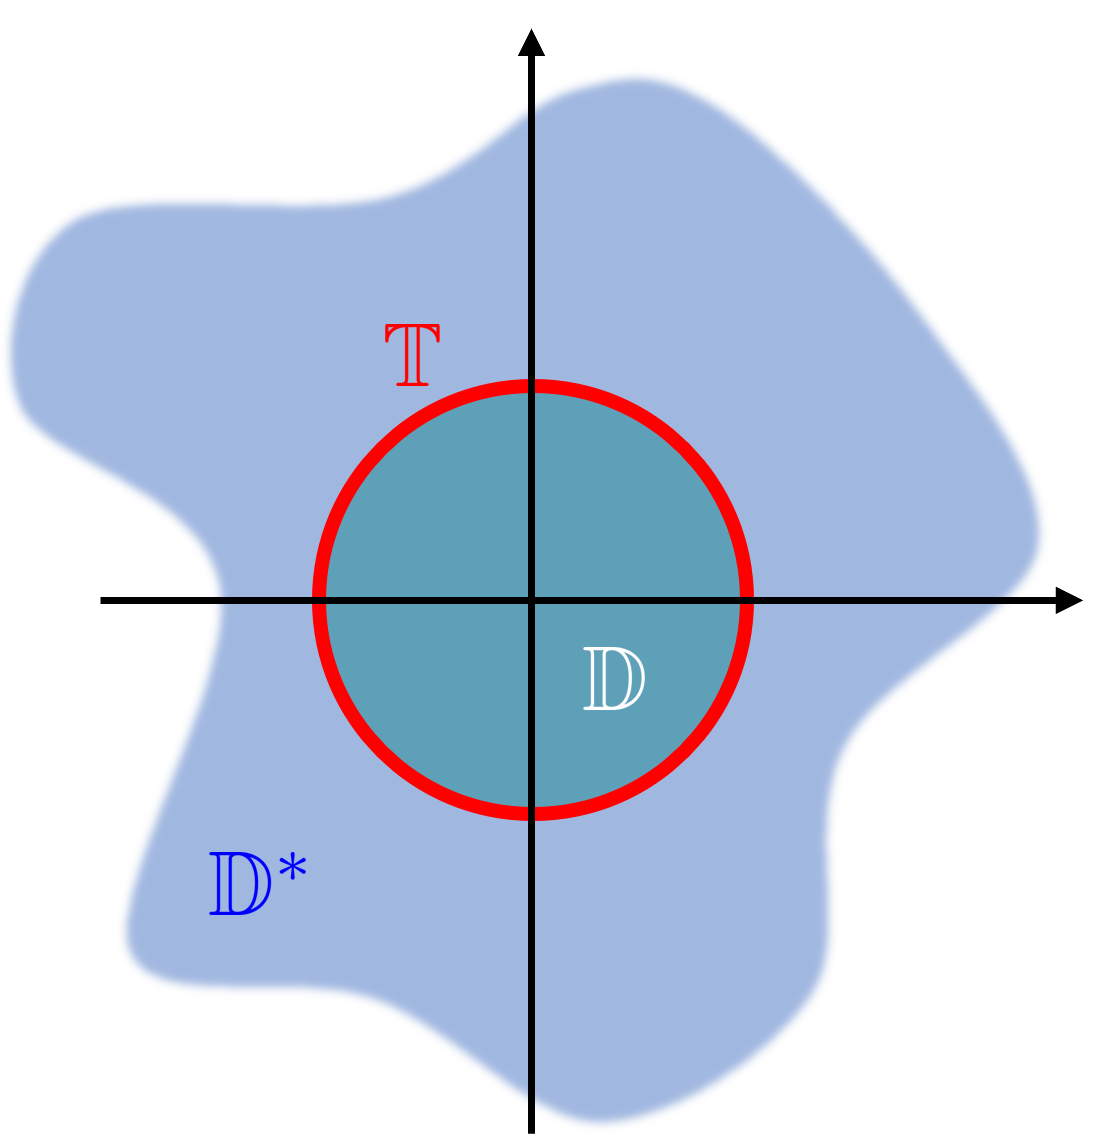
\includegraphics[width=0.8\linewidth]{figures/complex_plane.png}
            % \caption{Caption}
            % \label{fig:enter-label}
        \end{figure}
    \end{column}
    \end{columns}
\end{frame}
\begin{frame}{QSP \& NLFT}
    Immediately, let us link the two disparate mathematical fields: let $x=\cos\theta$, $z = \ee^{\ii2\theta}$, and $F_k = \ii\tan\phi_k$. Then since
    \begin{align}
        &W(x) = {\color{red}\ee^{\ii\theta X}}, & \frac{1}{\sqrt{1+\abs{F_k}^2}}\left[\begin{matrix}
            1 & F_kz^k \\ -\overline{F}_kz^{-k} & 1
        \end{matrix}\right] = \ee^{\ii k\theta Z} \ee^{\ii\phi_kX} \ee^{-\ii k\theta Z},
    \end{align}
    we have, for $F=(F_0,F_1,\ldots,F_n)$,
    \begin{align*}
        H V_\Phi(x) H &= H \ee^{\ii\phi_0Z} {\color{red}\ee^{i\theta X}} \ee^{\ii\phi_1Z} {\color{red}\ee^{i\theta X}} \cdots {\color{red}\ee^{i\theta X}} \ee^{\ii\phi_nZ} H \\
        &= H \ee^{\ii\phi_0Z} HH \ee^{i\theta X} HH \ee^{\ii\phi_1Z} HH \ee^{i\theta X} H\cdots H \ee^{i\theta X} HH \ee^{\ii\phi_nZ} H \\
        &= \ee^{\ii\phi_0\color{blue}X} \ee^{i\theta \color{blue}Z} \ee^{\ii\phi_1\color{blue}X} \ee^{i\theta \color{blue}Z} \cdots \ee^{i\theta \color{blue}Z} \ee^{\ii\phi_n\color{blue}X} \\
        &= \ee^{\ii\phi_0X}\left(\ee^{\ii\theta Z} \ee^{\ii\phi_1X} \ee^{-\ii\theta Z}\right) \left(\ee^{\ii2\theta Z} \cdots\right) \left(\ee^{\ii n\theta Z} \ee^{\ii\phi_nX}\ee^{-\ii n\theta Z}\right) \ee^{\ii n\theta Z} \\
        &= \mathcal{F}(z) \ee^{\ii n\theta Z}. \QED
    \end{align*}
\end{frame}

%%%%%%%%%%%%%%%%%%%%%%%%%%%%%%%%%%%%%%%%%%%%%%%%%%%%%%%%

\subsection{Prior Works}
\begin{frame}{Prior Works -- Layer-Stripping}
    Before we discuss how NLFT aids in our goal of QSP, let us review some history in the development of phase finding in QSP.

    We have seen the \textit{\color{blue}layer-stripping method} as introduced in \cite{GSLW18} in course:
    \begin{equation*}
        \left[\begin{matrix}
            P'(x) & * \\
            \ii\sqrt{1-x^2}Q'^*(x) & *
        \end{matrix}\right] = \left[\begin{matrix}
            P(x) & * \\
            \ii\sqrt{1-x^2}Q^*(x) & *
        \end{matrix}\right] \ee^{-\ii\phi_nZ} W^\dagger(x),
    \end{equation*}
    then
    \begin{equation*}
        P'(x) = \ee^{-\ii\phi_n}x\underbrace{P(x)}_{p_{n}x^{n}+\cdots} + \ee^{\ii\phi_n}(1-x^2)\underbrace{Q(x)}_{q_{n-1}x^{n-1}+\cdots}
    \end{equation*}
    reduces its order if and only if $\ee^{\ii2\phi_n} = p_{n} / q_{n-1}$.

    \color{red}However, this method is numerically unstable! \color{black}(Or is it?)
\end{frame}
\begin{frame}{Prior Works -- Layer-Stripping}
    Let us analyze the complexity to the layer-stripping method:
    \begin{itemize}
        \item The amount of FLOPs required is
        \begin{equation*}
            \underbrace{O(n)}_{n\text{ phase terms}} \cdot \underbrace{O(n)}_{P\text{ to }P'} = O(n^2).
        \end{equation*}
        \item For each computation, $\Theta(n \log(n/\varepsilon))$ bits of precision is required \cite{Haah_2019} such that $\norm{P - \hat{P}}_\infty < \varepsilon$.
    \end{itemize}

    The definition to a \textit{numerically stable} algorithm is its required number of bits is of order $\color{red} O(\polylog(n/\varepsilon))$.

    In \cite{Lin2025}, however, it is shown that stability can be achieved for certain $a$'s ({\color{red}outer}).
\end{frame}

\begin{frame}{Prior Works}
    Other methods were developed, such as: root finding, Prony's method \cite{Prony}, iterative optimization methods.
    
    But before any of that, we should ask ourselves whether the solution is unique? Many weird behaviors in the phase finding of QSP are discussed in \cite{EnergyLandscpae}. Consider requiring $f$ to be \textit{\color{red}real}\footnote{This constraint can be lifted.\vspace{2.5ex}}. Due to the parity constraint on $P$ being a real degree $n=2d$ even polynomial, we only have $d+1$ degrees of freedom. Hence, we should expect
    \begin{equation}
        \Phi= (\psi_{\color{red}d},\ldots,\psi_{\color{red}1},\underbrace{\psi_0,\psi_1,\ldots,\psi_d}_{\Psi})
    \end{equation}
    to be a symmetric phase $\Psi$. In the case of symmetric phase, we denote $V_\Phi=V_\Psi$, and this becomes the study of \textit{symmetric QSP}.
\end{frame}

\begin{frame}{Prior Works -- Iteration Methods}
    Iterative methods were proposed: consider the following optimization problem
    \begin{equation}
        \Psi^* = \arg\min_\Psi \norm{\hat{P}_\Psi - P}_2^2 = \arg\min_\Psi \sum_{k=1}^{d} \abs{\hat{P}_\Psi(x_k) - P(x_k)}^2,
    \end{equation}
    where $P$ is the function obtained from the QSP protocol with symmetric phase $\Psi$, and $x_k$ are the Chebyshev nodes. We can optimize via
    \begin{columns}
    \begin{column}{0.45\textwidth}
        \begin{enumerate}
            \item Fixed-point iteration \cite{FPI}:
            \begin{equation*}
                \Psi \mapsto \Psi - \frac{1}{2}(\hat{P}_\Psi - P).
            \end{equation*}
            Note that $\mathrm{D}\hat{P}_\Psi(0) = 2\mathbbm{1}$.
        \end{enumerate}
    \end{column}
    \begin{column}{0.45\textwidth}
        \begin{enumerate}
            \setcounter{enumi}{1}
            \item Newton's method \cite{Newton}:
            \begin{equation*}
                \Psi \mapsto \Psi - \underbrace{\mathrm{D}\hat{P}_\Psi^{-1}}_{\mathrm{Hess}^{-1}}\underbrace{(\hat{P}_\Psi-P)}_{\mathrm{grad}}.
            \end{equation*}
            \vspace{0.2em}
        \end{enumerate}
    \end{column}
    \end{columns}
\end{frame}

\begin{frame}{Prior Works -- Maximal Solution}
    \begin{columns}
    \begin{column}{0.4\textwidth}
        Even with the phase reduced, we cannot ensure our iterations converge. In fact, in \cite{EnergyLandscpae}, it is observed that there are multiple local minimas!

        \vspace{1em}
        
        There exists a global minima near the special initial condition $\Psi_0 = (0,\ldots,0)$. This solution is termed the \textit{\color{red}maximal solution}.
    \end{column}
    \begin{column}{0.5\textwidth}
        \begin{figure}
            \centering
            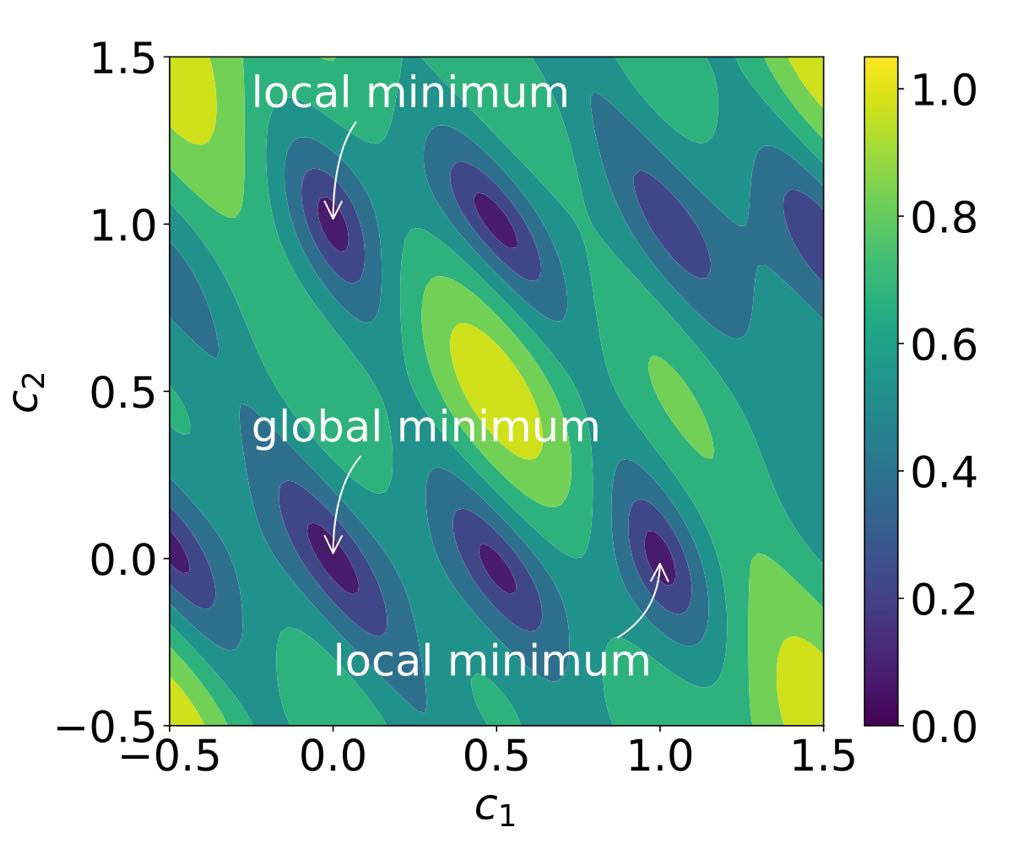
\includegraphics[width=1\linewidth]{figures/energy_landscape.jpg}
        \end{figure}
    \end{column}
    \end{columns}
\end{frame}

\begin{frame}{Prior Works -- Complexity Comparison}
    A summary of existing algorithms for inverse NLFT is as below:
    \begin{table}
        % \color{green}[need to check correctness]
        \centering
        \begin{tabular}{|c||c|c|c|}
            \hline
            Algorithm & Time Complexity\footnote{The algorithms with $^*$ requires the Weiss algorithm, costing an additional $O(n\polylog (n/\varepsilon))$.} & Coherence\footnote{$\norm{f}_\infty = 1-\eta$. If $\eta\sim0$, it is fully-coherent.\vspace{2.5ex}} & Stability\\ \hline\hline
            FPI \cite{FPI} & $\tilde{O}(n^2\log\varepsilon^{-1})$ & $1-\eta\ll1$ & Y \\
            FFPI \cite{half-cholesky} & $O(n\log^2n\log\varepsilon^{-1})$ & $1-\eta\ll1$ & Y \\ \hline
            Layer-Stripping \cite{Tsai} & $O(n^2)^*$ & Full & N/Y \\
            RHW \cite{Szego} & $O(n^4)^*$ & Full & Y \\ 
            HC \cite{half-cholesky} & $O(n^2)^*$ & Full & Y \\ \hline
            iNLFFT \cite{Lin2025} & ${\color{red}O(n\log^2n)}^*$ & Full & Y \\ \hline
        \end{tabular}
    \end{table}
\end{frame}



% \subsection{Mathematical Preliminaries}

% \begin{frame}{Hardy Function}
%     Holomorphic (analytic) functions that are $L^2$ on $\mathbb{T}$ are denoted by $\mathcal{H}^2(\mathbb{T})$, a \textit{Hardy} space.

%     We can extend the domain of the function to the complex plane while hoping that it remains analytic.
%     \begin{itemize}
%         \item If analytic continued onto $\mathbb{D}$, the function is in $\mathcal{H}^2(\mathbb{D})$, the function is of the form
%         \begin{equation*}
%             a(z) = a_0 + a_1z + a_2z^2 + \cdots.
%         \end{equation*}
%         \item If analytic continued onto $\mathbb{D}^*$, the function is in $\mathcal{H}^2(\mathbb{D}^*)$, the function is of the form
%         \begin{equation*}
%             a(z) = a_0 + a_1z^{\color{red}-1} + a_2z^{\color{red}-2} + \cdots.
%         \end{equation*}
%     \end{itemize}
% \end{frame}


